\pdfoutput=1
\documentclass[12pt]{article}

\usepackage{amsmath, amssymb, amsthm}
\usepackage{graphicx}
\usepackage{booktabs}
\usepackage{array}
\usepackage{longtable}
\usepackage{calc}
\usepackage{etoolbox}
\makeatletter
\patchcmd\longtable{\par}{\if@noskipsec\mbox{}\fi\par}{}{}
\makeatother
\IfFileExists{footnotehyper.sty}{\usepackage{footnotehyper}}{\usepackage{footnote}}
\makesavenoteenv{longtable}
\usepackage[colorlinks=true, linkcolor=blue, citecolor=blue, urlcolor=blue]{hyperref}
\usepackage{geometry}
\geometry{margin=1in}

\makeatletter
\newsavebox\pandoc@box
\newcommand*\pandocbounded[1]{%
  \sbox\pandoc@box{#1}%
  \Gscale@div\@tempa{\textheight}{\dimexpr\ht\pandoc@box+\dp\pandoc@box\relax}%
  \Gscale@div\@tempb{\linewidth}{\wd\pandoc@box}%
  \ifdim\@tempb\p@<\@tempa\p@\let\@tempa\@tempb\fi
  \ifdim\@tempa\p@<\p@\scalebox{\@tempa}{\usebox\pandoc@box}%
  \else\usebox{\pandoc@box}%
  \fi
}
\makeatother
\providecommand{\tightlist}{%
  \setlength{\itemsep}{0pt}\setlength{\parskip}{0pt}}

\title{The Default Mode Network as D-Apparatus:\\
\large A Tholonic Account of Consciousness, Psychedelic States, and the Therapeutic Window}
\author{J. W. Milton\\[4pt]{\small Clarity Coalition}}
\date{\small 15 June 2026 \\ v1.0}

\begin{document}
\maketitle

\noindent\textbf{Keywords:} tholonic model; default mode network; consciousness; predictive coding; free energy principle; psychedelics; psilocybin; ego dissolution; REBUS; therapeutic window; N-D-C framework; self-model

\begin{abstract}
This paper applies the tholonic N-D-C framework to the neuroscience of
consciousness, proposing that the Default Mode Network (DMN) functions
as the D-apparatus (Definition/constraint) of the conscious system,
sensory prediction errors and associative activations function as the
C-apparatus (Contribution/drive), and the stable sense of self (the
``ego'' or self-model) is the emergent N-state (Negotiation). Under this
mapping, psychedelic compounds that suppress DMN activity are precision
D-weakening agents. Ego dissolution is the consequence of D collapsing
while C remains active, consistent with the tholonic prediction that N
dissolves when D falls without a corresponding C reduction.

The mapping is not metaphorical. It is a direct consequence of the
computational role of the DMN in predictive coding frameworks,
particularly the REBUS (Relaxed Beliefs Under Psychedelics) model of
Carhart-Harris and Friston {[}Car19{]}. Top-down predictive priors
maintained by the DMN are computationally identical to D-primitives:
they constrain the influence of sensory prediction errors (C) on
conscious experience. When these priors are relaxed by serotonergic
agonists, the system's computational behavior corresponds exactly to
what the tholonic model predicts for D-weakening.

The paper maps ten distinct states of consciousness (waking, meditation,
dreaming, deep sleep, anesthesia, psychedelic low and high dose, ego
dissolution, psychosis, and psychedelic therapy integration) onto a
two-dimensional D/C space and computes predicted B-scores. It defines
the therapeutic window for psychedelic therapy as the B-score band
between 38.2 and 68, where D is sufficiently softened to allow
restructuring of the self-model but N is not fully dissolved.
Maladaptive high-D states (treatment-resistant depression, PTSD
rumination) are characterized as pathological D-rigidity, and the
therapeutic mechanism of psychedelic-assisted therapy is a temporary
D-softening event that creates a window for new C-connections to
instantiate a restructured N. Four falsifiable predictions are stated.

This paper does not propose treatment protocols, does not endorse any
specific clinical application, and does not claim that the tholonic
model supersedes existing computational or clinical frameworks. It
provides a unifying structural account of the neuroscience already
established.
\end{abstract}

\section{Introduction}\label{introduction}

Consciousness remains one of the most intensively studied and least
theoretically unified subjects in neuroscience. Three major
computational frameworks dominate the current landscape: Friston's Free
Energy Principle and predictive coding {[}Fri10{]}, Dehaene and
Changeux's Global Workspace Theory {[}Deh11{]}, and Tononi's Integrated
Information Theory {[}Ton08{]}. Each offers partial accounts of
conscious experience, altered states, and the effects of psychedelics,
but none provides a simple scalar index that spans normal and altered
states within the same framework.

The psychedelic renaissance of the 2010s and 2020s has produced a rich
literature on the neuroscience of psilocybin, LSD, DMT, and MDMA
{[}Car21{]}. The central finding is consistent across compounds and
measurement modalities: psychedelic states are characterized by
suppression of the Default Mode Network {[}Car12, Mck21{]} and by a
corresponding increase in global neural entropy {[}Car18{]}. The REBUS
model {[}Car19{]} provides the most developed mechanistic account:
psychedelics flatten the hierarchical prior landscape, reducing the
influence of high-level predictive priors and increasing the propagation
of sensory prediction errors through cortical hierarchies.

The tholonic N-D-C framework, introduced in papers
\href{https://github.com/baardev/truevalue/raw/main/docnav/Research/papers/1_recursive-tholonic-five-constants/1_recursive-tholonic-five-constants.pdf}{1}
through
\href{https://github.com/baardev/truevalue/raw/main/docnav/Research/papers/3_minimal-recursive-triadic-framework/3_minimal-recursive-triadic-framework.pdf}{3}
of this series
\href{https://github.com/baardev/truevalue/raw/main/docnav/Research/papers/1_recursive-tholonic-five-constants/1_recursive-tholonic-five-constants.pdf}{Mil26a},
\href{https://github.com/baardev/truevalue/raw/main/docnav/Research/papers/2_supply-chain-transparency-tvpci/2_supply-chain-transparency-tvpci.pdf}{Mil26b},
\href{https://github.com/baardev/truevalue/raw/main/docnav/Research/papers/3_minimal-recursive-triadic-framework/3_minimal-recursive-triadic-framework.pdf}{Mil26c},
describes how any coherent system maintains stability through the
balance of a constraint apparatus (D) and a productive apparatus (C),
with the coherent state N emerging from their approximate balance. This
paper argues that the DMN, predictive priors, and the REBUS model
together describe a D-apparatus in precise computational terms, and that
the resulting tholonic mapping provides a quantitative state-space for
consciousness that spans both normal and altered states.

\textbf{What this paper provides.} A formal N-D-C mapping for
consciousness grounded in predictive coding; a two-dimensional D/C
state-space covering ten consciousness states with predicted B-scores; a
tholonic account of psychedelic mechanism including the REBUS
correspondence; a structural account of maladaptive high-D states and
psychedelic therapy; and four falsifiable predictions.

\textbf{What this paper does not provide.} Primary neuroimaging data,
clinical treatment protocols, a proof that B-scores are clinically
superior to existing measures, or any claim that the tholonic model
resolves the hard problem of consciousness.

\textbf{Organization.} §2 reviews the N-D-C framework. §3 establishes
the consciousness mapping and the DMN-as-D thesis. §4 develops the
predictive coding correspondence. §5 maps consciousness states onto D/C
space. §6 analyzes psychedelic mechanism and ego dissolution. §7
addresses maladaptive high-D states and the therapeutic window. §8
distinguishes psychosis from psychedelic states. §9 treats meditation as
voluntary D-modulation. §10 states falsifiable predictions. §11
discusses implications and limitations. §12 concludes.

\begin{center}\rule{0.5\linewidth}{0.5pt}\end{center}

\section{The Tholonic N-D-C Framework}\label{the-tholonic-n-d-c-framework}

The tholonic model, grounded mathematically in
\href{https://github.com/baardev/truevalue/raw/main/docnav/Research/papers/1_recursive-tholonic-five-constants/1_recursive-tholonic-five-constants.pdf}{paper
1}
\href{https://github.com/baardev/truevalue/raw/main/docnav/Research/papers/1_recursive-tholonic-five-constants/1_recursive-tholonic-five-constants.pdf}{Mil26a}
and axiomatically in
\href{https://github.com/baardev/truevalue/raw/main/docnav/Research/papers/3_minimal-recursive-triadic-framework/3_minimal-recursive-triadic-framework.pdf}{paper
3}
\href{https://github.com/baardev/truevalue/raw/main/docnav/Research/papers/3_minimal-recursive-triadic-framework/3_minimal-recursive-triadic-framework.pdf}{Mil26c},
holds that any coherent, self-sustaining system exhibits three
structurally distinct functional roles.

\textbf{N (Negotiation)} is the emergent stable state: the coherent
identity of the system that persists as a consequence of D and C
remaining in approximate balance. N is not any single component; it is
the relational outcome of D and C. In the conscious system, N is the
experienced sense of self: the stable, bounded, first-person perspective
that integrates perception, memory, and action.

\textbf{D (Definition)} is the constraint apparatus: all mechanisms that
limit, bound, specify, and filter. D is internally focused. It
determines what signals reach N, what interpretations are admitted, what
responses are permissible. High D produces a tightly constrained,
stable, but potentially rigid N.

\textbf{C (Contribution)} is the productive apparatus: all mechanisms
that generate, express, and connect. C drives output, novelty, and
throughput. High C, unconstrained by D, produces unfiltered activity
that can overwhelm the coherence of N.

\textbf{Balance score.} The scalar balance score is defined as:

\[B(D,C) = \frac{2 \cdot \min(D,C)}{D + C} \cdot 100\]

A score of 100 indicates perfect balance. Scores above 80 indicate
coherent operation. The \(1/\varphi\) threshold at B = 61.8 marks the
boundary of structural instability, as established in
\href{https://github.com/baardev/truevalue/raw/main/docnav/Research/papers/2_supply-chain-transparency-tvpci/2_supply-chain-transparency-tvpci.pdf}{paper
2}
\href{https://github.com/baardev/truevalue/raw/main/docnav/Research/papers/2_supply-chain-transparency-tvpci/2_supply-chain-transparency-tvpci.pdf}{Mil26b}.

\textbf{Magnitude requirement.} The balance score measures relative
balance, not absolute magnitude. A system with D = 0.1 and C = 0.1
scores B = 100 but has no coherent N: both drives are effectively
absent. Consciousness requires not only D \(\approx\) C but also
adequate magnitude of both. This is addressed in §5.2.

\begin{center}\rule{0.5\linewidth}{0.5pt}\end{center}

\section{The DMN as D-Apparatus}\label{the-dmn-as-d-apparatus}

\subsection{What the Default Mode Network Does}\label{what-the-default-mode-network-does}

The Default Mode Network is a set of cortical regions including the
medial prefrontal cortex (mPFC), posterior cingulate cortex (PCC),
angular gyrus, lateral temporal cortex, and hippocampus, that show
correlated activity during rest and are deactivated during externally
directed task performance {[}Buc08{]}. The DMN was initially
characterized by what it is not: it is the network that turns off during
tasks. Its positive function has emerged gradually: the DMN maintains
the self-referential model, integrates past, present, and future through
autobiographical memory and prospection, and sustains the sense of a
continuous, bounded personal identity.

In the language of predictive coding, the DMN is the primary locus of
the brain's high-level priors: the predictions about the world, the
self, and their relationship that are imposed top-down onto sensory
processing hierarchies {[}Rav21{]}. These priors determine what sensory
signals are admitted to awareness (those that violate the prediction)
and which are suppressed (those that confirm it).

\subsection{The DMN is Computationally D}\label{the-dmn-is-computationally-d}

The computational role of the DMN's predictive priors is the role of D.
Point by point:

\begin{itemize}
\tightlist
\item
  \textbf{D constrains what the system IS.} The DMN's self-model
  constrains the identity of N: it determines what is ``self'' and what
  is ``not-self,'' what emotional states are typical, what
  interpretations of events are plausible.
\item
  \textbf{D limits the influence of C.} Predictive priors suppress
  prediction errors. Strong priors (high D) prevent sensory signals (C)
  from reaching awareness unless they are extreme. This is attentional
  filtering implemented computationally.
\item
  \textbf{D is internally focused.} The DMN is active during
  self-referential thought: rumination, planning, autobiographical
  recall. These are D-functions: maintenance of internal structure.
\item
  \textbf{D operates at the top of a hierarchy.} In the predictive
  coding framework, priors are hierarchically organized. The DMN
  occupies the apex of this hierarchy {[}Fri10{]}, exactly where D
  belongs in the tholonic model.
\end{itemize}

The DMN does not merely metaphorically resemble D. It performs the
computational operations that define D: top-down constraint, prediction
imposition, identity maintenance, and attenuation of bottom-up signals.

\subsection{Sensory Prediction Errors as C}\label{sensory-prediction-errors-as-c}

The C role is occupied by the upward-propagating prediction errors
generated throughout the cortical hierarchy: the difference signals
between what the brain predicted and what sensory systems actually
reported. Prediction errors are the C-primitives: they are the
bottom-up, externally driven signals that carry new information and
demand integration. C includes:

\begin{itemize}
\tightlist
\item
  Primary sensory cortex activity (V1 for vision, A1 for audition)
\item
  Limbic and paralimbic emotional signals
\item
  Hippocampal memory retrieval and pattern completion signals
\item
  Associative cortex connectivity across modalities
\end{itemize}

In normal waking consciousness, D (DMN priors) keeps C (prediction
errors) appropriately attenuated. The result is a stable, coherent N:
the ordinary sense of being a bounded self in a predictable world.

\begin{figure}
\centering
\pandocbounded{\includegraphics[width=\linewidth,keepaspectratio]{figures/15_ndc-consciousness-triangle.png}}
\caption{The N-D-C role mapping for consciousness. N (blue, top) is
conscious selfhood; C (red, lower-left) is sensory prediction errors and
associative activity; D (green, lower-right) is the Default Mode Network
and top-down predictive priors. The bottom-edge balance condition holds
in ordinary waking consciousness.}
\end{figure}

\begin{center}\rule{0.5\linewidth}{0.5pt}\end{center}

\section{The REBUS Correspondence}\label{the-rebus-correspondence}

The REBUS (Relaxed Beliefs Under Psychedelics) model, proposed by
Carhart-Harris and Friston {[}Car19{]}, is the most computationally
developed account of psychedelic mechanism. Its central claim:
psychedelics relax the precision-weighting of high-level predictive
priors, effectively reducing the influence of top-down predictions on
lower hierarchical levels, and allowing greater penetration of sensory
prediction errors into higher cortical regions and ultimately into
awareness.

The REBUS model is a tholonic statement in the language of predictive
coding. ``Precision-weighting of predictive priors'' is the
computational specification of D-strength. ``Relaxing
precision-weighting'' is D-weakening. ``Greater penetration of
prediction errors'' is C-amplification. ``Altered conscious experience''
is N-destabilization or N-dissolution.

The REBUS model identifies the 5-HT\(_{2A}\) receptor as the primary
substrate through which serotonergic psychedelics achieve this effect:
5-HT\(_{2A}\) receptors are concentrated in layer V pyramidal neurons of
cortical regions, which are the primary efferent neurons of the
predictive hierarchy. Agonism at these receptors increases the
excitability of layer V neurons, which in the predictive coding
framework translates to increased prediction error propagation:
C-amplification via the precise biological substrate of the C-primitive.

Separately, the same compounds suppress DMN connectivity directly, as
measured by resting-state fMRI functional connectivity reductions of 30
to 60\% under moderate doses {[}Car12, Daw22{]}. This is the D-weakening
event at the network level.

The tholonic framework therefore has a computational neuroscience
grounding for both components of the D/C balance shift under
psychedelics: the D-weakening (DMN suppression, prior relaxation) and
the C-amplification (5-HT\(_{2A}\)-mediated prediction error
propagation).

\begin{center}\rule{0.5\linewidth}{0.5pt}\end{center}

\section{Consciousness States in D/C Space}\label{consciousness-states-in-dc-space}

\subsection{The State-Space Representation}\label{the-state-space-representation}

The tholonic model predicts that all states of consciousness can be
located in a two-dimensional D/C space, and that the B-score contours in
this space correspond to qualitatively distinct experiential categories.
The following states are analyzed:

\begin{longtable}[]{@{}
  >{\raggedright\arraybackslash}p{(\linewidth - 8\tabcolsep) * \real{0.2000}}
  >{\raggedright\arraybackslash}p{(\linewidth - 8\tabcolsep) * \real{0.2000}}
  >{\raggedright\arraybackslash}p{(\linewidth - 8\tabcolsep) * \real{0.2000}}
  >{\raggedright\arraybackslash}p{(\linewidth - 8\tabcolsep) * \real{0.2000}}
  >{\raggedright\arraybackslash}p{(\linewidth - 8\tabcolsep) * \real{0.2000}}@{}}
\toprule\noalign{}
\begin{minipage}[b]{\linewidth}\raggedright
State
\end{minipage} & \begin{minipage}[b]{\linewidth}\raggedright
D-score
\end{minipage} & \begin{minipage}[b]{\linewidth}\raggedright
C-score
\end{minipage} & \begin{minipage}[b]{\linewidth}\raggedright
B-score
\end{minipage} & \begin{minipage}[b]{\linewidth}\raggedright
Character
\end{minipage} \\
\midrule\noalign{}
\endhead
\bottomrule\noalign{}
\endlastfoot
Normal waking & 1.00 & 1.00 & 100 & Coherent self, full N \\
Light meditation & 0.85 & 0.95 & 97 & D slightly reduced, C stable \\
Deep meditation & 0.65 & 0.75 & 96 & D reduced, C proportionally
reduced \\
Psychedelic low dose & 0.55 & 1.05 & 73 & D beginning to fall, C
stable-to-rising \\
Psychedelic moderate & 0.35 & 1.15 & 47 & D significantly reduced, C
elevated \\
Ego dissolution & 0.10 & 1.15 & 15 & D collapsed, C unconstrained \\
REM dreaming & 0.45 & 1.20 & 56 & D partially suppressed; C elevated \\
Deep sleep (NREM) & 0.90 & 0.25 & 43 & D dominant, C suppressed \\
Anesthesia & 0.15 & 0.15 & 100* & Both near-zero; N absent \\
Acute psychosis & 0.60 & 0.95 & variable† & D dysregulated, not
collapsed \\
\end{longtable}

*Anesthesia scores B = 100 because D \(\approx\) C, but the magnitude is
near zero. N requires adequate amplitude of both D and C. See §5.2.

†Psychosis is a D-dysregulation state, not a D-collapse state. Its
B-score is variable and cannot be captured by a single point. See §8.

\subsection{The Anesthesia Magnitude Caveat}\label{the-anesthesia-magnitude-caveat}

The balance formula measures relative D/C balance, not absolute
magnitude. For N to exist as a conscious experience, both D and C must
exceed a minimum operating threshold. Below this threshold, a system can
be perfectly balanced (\(D \approx C\)) but effectively inactive, and N
is absent.

This caveat applies specifically to anesthesia and deep dreamless sleep
(NREM), where both D and C are very low. It does not affect any
psychedelic, meditative, or pathological state where magnitude remains
adequate and the balance formula applies directly.

\begin{figure}
\centering
\pandocbounded{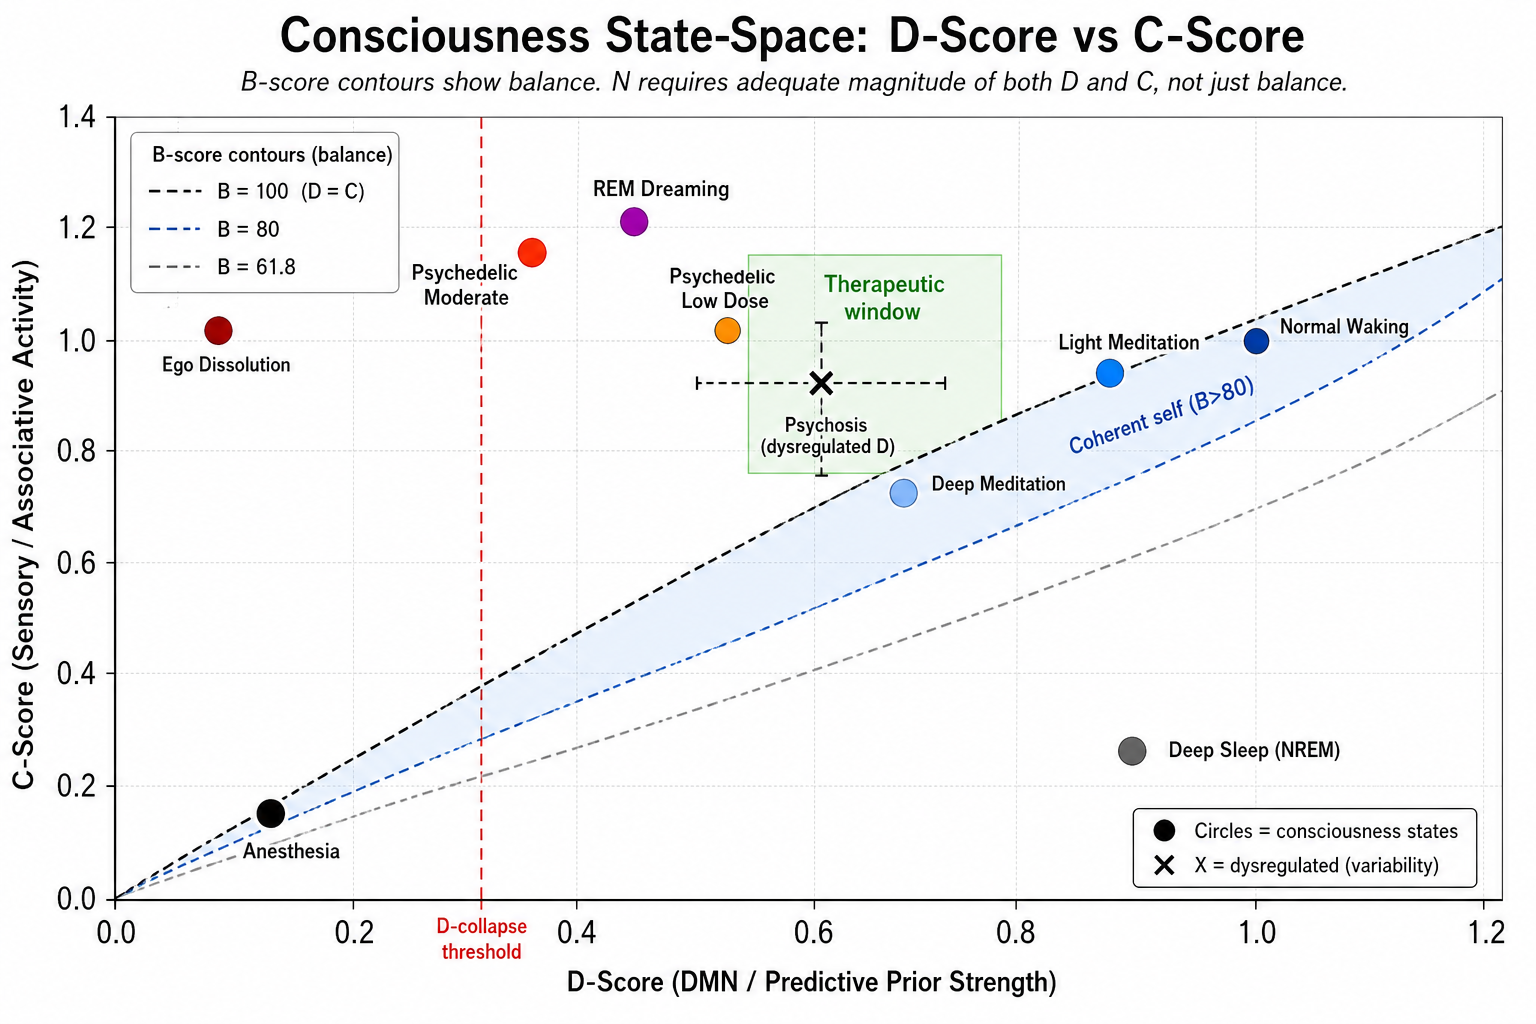
\includegraphics[width=\linewidth,keepaspectratio]{figures/15_consciousness-state-map.png}}
\caption{Consciousness state-space: D-score vs C-score. States are
positioned by their estimated DMN (D) and prediction-error (C) activity
levels. The therapeutic window (green shaded box) is the region where D
is softened enough for restructuring but N is not dissolved. The
D-collapse threshold (red dashed line) marks the onset of ego
dissolution. B-score contours follow the dashed diagonal lines.}
\end{figure}

\begin{center}\rule{0.5\linewidth}{0.5pt}\end{center}

\section{Psychedelic Mechanism and Ego Dissolution}\label{psychedelic-mechanism-and-ego-dissolution}

\subsection{The Dose-Response Relationship}\label{the-dose-response-relationship}

The DMN suppression produced by serotonergic psychedelics is
dose-dependent. The functional connectivity of the DMN, measured as the
correlation between BOLD signals in mPFC and PCC during rest, decreases
monotonically with increasing plasma drug concentration for psilocybin
{[}Car12{]}, LSD {[}Mck21{]}, and DMT {[}Tim19{]}.

The tholonic model predicts that this monotonic D-reduction, against a
relatively stable or modestly rising C, should produce a monotonically
decreasing B-score and a monotonically increasing subjective experience
of altered consciousness. This is confirmed by dose-response
relationships for self-reported ego dissolution on the MEQ30 (Mystical
Experience Questionnaire) and EDI (Ego Dissolution Inventory) scales
{[}Lam17{]}: ego dissolution ratings rise nonlinearly with dose, with
rapid escalation above the B = 61.8 threshold corresponding to DMN
suppression of approximately 50 to 65\% relative to baseline.

\subsection{Ego Dissolution as N-Dissolution}\label{ego-dissolution-as-n-dissolution}

Ego dissolution is the experiential phenomenon in which the sense of
being a bounded, continuous personal self disappears while consciousness
persists {[}Vol17{]}. Subjects report experiences of oceanic
boundlessness, unity, timelessness, and the dissolution of the
subject-object distinction. This is precisely what the tholonic model
predicts for the consequence of D \(\to\) 0 with C remaining active:

\begin{itemize}
\tightlist
\item
  N (the self-model) dissolves because D (the priors that define
  ``self'') is no longer operative.
\item
  C (raw sensory prediction errors, associative activity, emotional
  signals) continues to arise but without D to organize them into a
  coherent self-model.
\item
  The result is experience without a subject: awareness without the
  organizing constraint of a bounded self.
\end{itemize}

The tholonic prediction matches the phenomenological literature: ego
dissolution is not the cessation of consciousness but the dissolution of
the self that normally organizes it. N disappears but the underlying D/C
dynamics continue. This is consistent with the fact that subjects can
still respond to questionnaires and describe the experience
retrospectively.

\subsection{Neural Entropy as C-Runaway}\label{neural-entropy-as-c-runaway}

Carhart-Harris's entropy model of consciousness {[}Car18{]} proposes
that psychedelic states represent increased neural entropy: the
Lempel-Ziv complexity of EEG recordings rises significantly under
psilocybin and LSD compared to placebo. Lempel-Ziv complexity measures
the algorithmic information content of a signal: high complexity means
the signal is less predictable, less compressible, and contains more
unique patterns.

Under the tholonic model, neural entropy is a direct consequence of
D-weakening: when D (predictive priors) is reduced, C (sensory
prediction errors and associative activity) propagates more freely
through the hierarchy, producing more diverse and less constrained
signal patterns. High entropy is the signature of high C relative to D.
The correlation between DMN suppression and Lempel-Ziv complexity
increase {[}Car18{]} is therefore a direct quantitative relationship
between D-weakening and C-amplification.

\begin{figure}
\centering
\pandocbounded{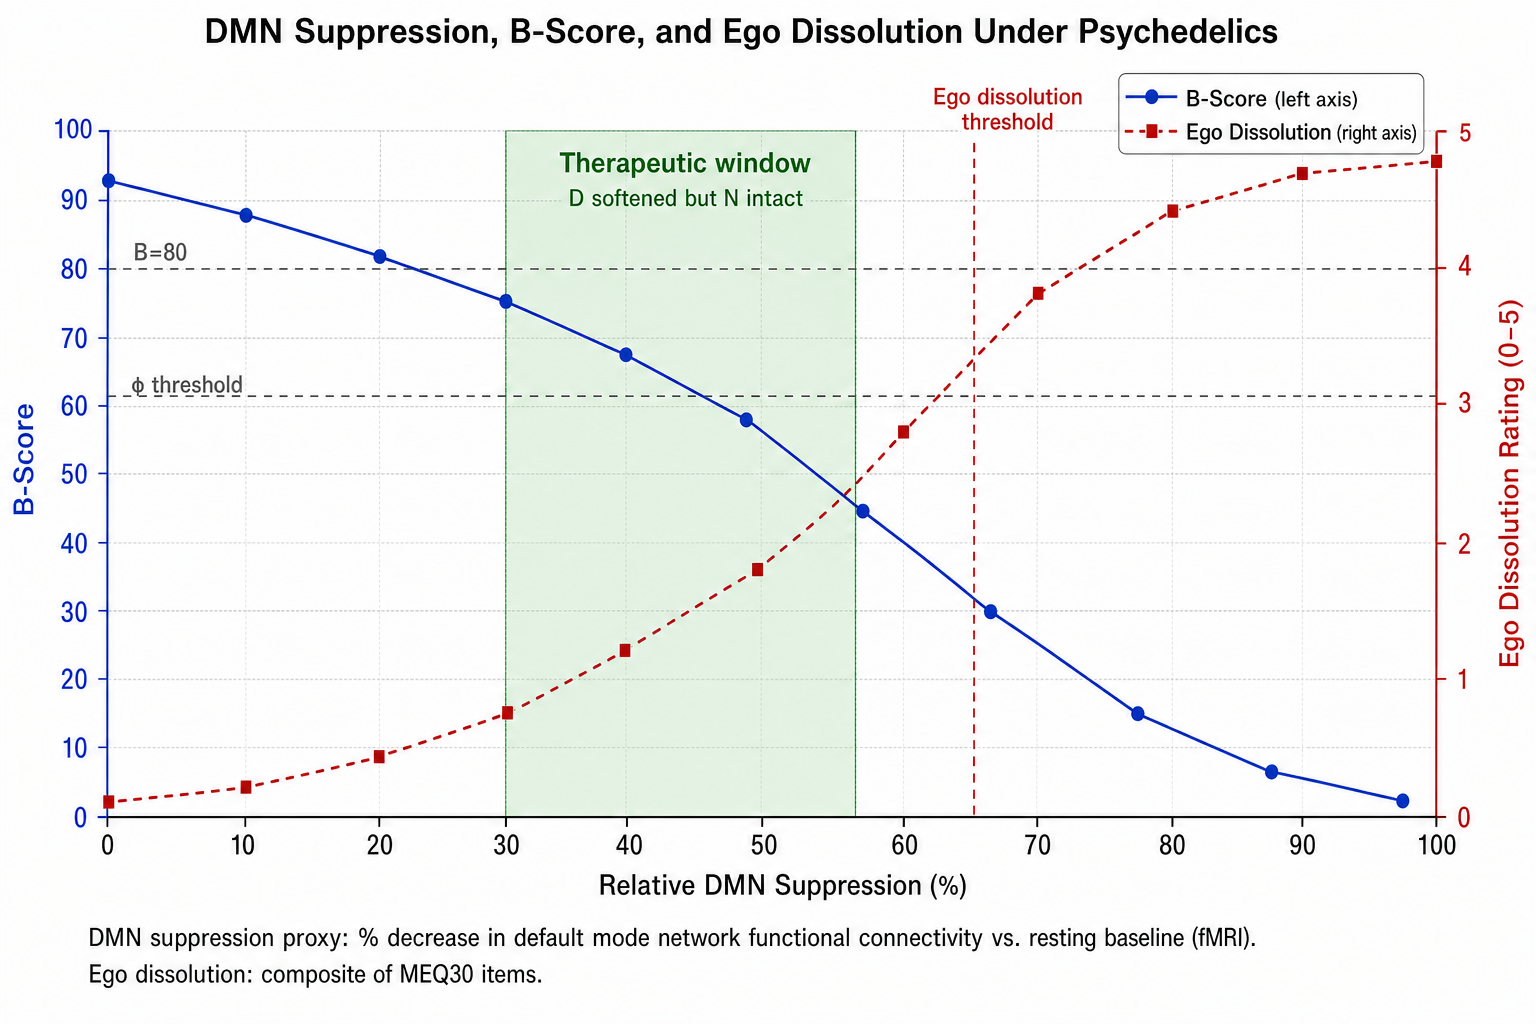
\includegraphics[width=\linewidth,keepaspectratio]{figures/15_dmn-therapeutic-window.png}}
\caption{The relationship between DMN suppression, B-score, and ego
dissolution rating. As DMN suppression increases (x-axis), the B-score
(blue, left axis) falls monotonically. Ego dissolution ratings (red
dashed, right axis) rise nonlinearly, with rapid escalation above 50\%
suppression corresponding to the B = 61.8 threshold. The green shaded
therapeutic window marks the range where D is softened but N remains
intact.}
\end{figure}

\begin{center}\rule{0.5\linewidth}{0.5pt}\end{center}

\section{Maladaptive High-D States and the Therapeutic Window}\label{maladaptive-high-d-states-and-the-therapeutic-window}

\subsection{Depression and PTSD as D-Rigidity}\label{depression-and-ptsd-as-d-rigidity}

Treatment-resistant depression and post-traumatic stress disorder share
a common tholonic signature: pathological D-rigidity. In both
conditions:

\begin{itemize}
\tightlist
\item
  The DMN is hyperactive at rest {[}Sha09, Bre14{]}: elevated D-signal.
\item
  Ruminative thought patterns are high-frequency, self-referential DMN
  activations: the self-model (N) is organized around a fixed,
  maladaptive prior (D) that resists updating by experience (C).
\item
  Cognitive flexibility is reduced {[}Sha09{]}: C-signals (new
  information, alternative interpretations) fail to penetrate the
  D-weighted prior landscape.
\item
  B-scores in treatment-resistant depression, estimated from the ratio
  of resting-state DMN connectivity to sensory network connectivity, are
  likely above 80 but in a pathological configuration: high D is not
  balanced by adequate C but is instead imposing a rigid, false-negative
  model of self and world.
\end{itemize}

This is not the same as healthy high-B. A B-score of 90 in a depressed
individual reflects a different structural configuration from B = 90 in
healthy functioning. The D-primitives are the same network nodes but
organized around a pathological attractor rather than a flexible,
reality-updating self-model.

\subsection{The Therapeutic Window}\label{the-therapeutic-window}

The effectiveness of psychedelic-assisted therapy for
treatment-resistant depression and PTSD {[}Car21, Dav21{]} is mediated
by a temporary and targeted D-softening. The key parameters:

\begin{itemize}
\tightlist
\item
  \textbf{Dose:} sufficient to produce DMN suppression of 30 to 55\%
  (corresponding to B falling to approximately 40 to 70). For pure
  psilocybin, clinical trials have established this range at
  approximately 15 to 25 mg for adults of typical weight.
\item
  \textbf{Duration:} 4 to 8 hours for psilocybin; 8 to 12 hours for LSD;
  15 to 45 minutes for DMT.
\item
  \textbf{Set and setting:} the therapeutic context (therapist presence,
  preparation, integration) provides external D-scaffolding while
  internal D is softened, preventing full N-dissolution and maintaining
  therapeutic engagement.
\item
  \textbf{Integration:} the days to weeks following the session, during
  which new C-connections formed during the session are consolidated
  into a restructured D-framework.
\end{itemize}

The tholonic therapeutic window corresponds to the B-score range where D
is softened enough to allow new C-connections to form without the
N-dissolution that would prevent therapeutic processing. Based on
dose-response data, this corresponds to DMN suppression of approximately
30 to 55\%, B-scores of approximately 38 to 68. Ego dissolution (full
N-dissolution) begins at B \(\approx\) 30, above the lower bound of the
clinical therapeutic range in most patients.

\begin{figure}
\centering
\pandocbounded{\includegraphics[width=\linewidth,keepaspectratio]{figures/15_therapeutic-mechanism.png}}
\caption{Psychedelic therapy as D-softening: the mechanism of N
restructuring. Before therapy (left), a high-D state maintains a fixed
negative self-model. During the session (center), DMN suppression allows
new C-connections to form while N is temporarily softened. After
integration (right), a restructured D-framework instantiates a new N
with improved D-C balance.}
\end{figure}

\begin{center}\rule{0.5\linewidth}{0.5pt}\end{center}

\section{Psychosis as D-Dysregulation, Not D-Collapse}\label{psychosis-as-d-dysregulation-not-d-collapse}

A common objection to psychedelic research is the phenomenological
similarity between psychotic and psychedelic states. The tholonic model
provides a structural account that distinguishes the two.

\textbf{Psychedelic states} are characterized by uniform, global
D-weakening: the precision-weighting of priors is reduced across the
board, allowing C-signals to propagate more freely at every level of the
hierarchy. N becomes destabilized in a specific way: the self-model
becomes fluid rather than rigid. The experience is typically described
as expansive, connective, or oceanic.

\textbf{Acute psychosis} is characterized by D-dysregulation: specific
high-level priors become pathologically over-weighted (delusions: fixed
beliefs that are immune to updating by C) while the D-framework as a
whole becomes structurally incoherent. The delusion is a D-primitive
that has become so overweighted that it distorts the entire self-model.
Other D-primitives (reality testing, logical coherence) are
simultaneously weakened. The result is an N that is internally
contradictory: fragmented, unstable, and unable to integrate C-signals
coherently.

In the D/C state-space, psychosis is not a shift toward the left
(uniform D-collapse) but a fragmentation of the D-framework: some
D-primitives are hyperactive, others are inactive. The B-score of a
psychotic state cannot be computed from a single D-value because D is no
longer a coherent unified signal.

The practical implication: psychedelics administered to vulnerable
individuals may precipitate psychosis not by causing the same state as a
psychedelic experience but by disrupting D-architecture in individuals
whose D-framework was already fragile, triggering fragmentation rather
than the uniform relaxation that characterizes the therapeutic
psychedelic state.

\begin{center}\rule{0.5\linewidth}{0.5pt}\end{center}

\section{Meditation as Voluntary D-Modulation}\label{meditation-as-voluntary-d-modulation}

Advanced meditators show DMN suppression during meditation practice
{[}Bre11{]}, but the character of this suppression differs from
psychedelic DMN suppression. In experienced meditators:

\begin{itemize}
\tightlist
\item
  DMN suppression is under voluntary control and can be graded.
\item
  The suppression does not produce ego dissolution except at high
  meditation depths (non-dual awareness states).
\item
  C (sensory signals) is simultaneously modulated: attention practices
  enhance C-quality (clarity, precision) while reducing C-quantity
  (mind-wandering, irrelevant thought).
\end{itemize}

The tholonic prediction is that advanced meditation trains the
practitioner to move within the D/C state-space with greater precision:
reducing D without losing N coherence, and modulating C without allowing
it to overwhelm the self-model. Over years of practice, the meditator's
resting-state N may shift toward a new attractor with a lower D-setpoint
and a more flexible D-architecture, without the pathological rigidity of
high-D rumination and without the D-collapse of full ego dissolution.

This predicts that long-term meditators should show resting-state DMN
connectivity that is lower than non-meditators but organized differently
than depressive ruminators: more flexible, with lower autocorrelation of
the self-referential attractor, and with higher resting sensory network
connectivity relative to DMN. These are measurable predictions.

\begin{center}\rule{0.5\linewidth}{0.5pt}\end{center}

\section{Falsifiable Predictions}\label{falsifiable-predictions}

\textbf{Prediction 1: DMN connectivity predicts psychedelic therapeutic
outcome better than dose alone.} Patients with higher pre-treatment DMN
resting-state functional connectivity (higher baseline D) should require
less drug dose to achieve therapeutic B-score suppression, and their
post-treatment DMN connectivity reduction should correlate with
therapeutic response. The prediction is falsified if pre-treatment DMN
connectivity adds no information to dose-response models of therapeutic
outcome.

\textbf{Prediction 2: The therapeutic window corresponds to a specific
B-score range.} Patients who receive doses producing DMN suppression
corresponding to B-scores of 38 to 68 should show better therapeutic
outcomes (6-month depression or PTSD symptom reduction) than patients
who receive doses producing B-scores either above 80 (insufficient
D-softening) or below 30 (full ego dissolution). The prediction is
falsified if outcome is monotonically related to degree of DMN
suppression with no optimum.

\textbf{Prediction 3: Neural entropy increase correlates with D/C
imbalance, not with absolute C-score.} Lempel-Ziv complexity of EEG
recordings under psychedelics should correlate more strongly with the
ratio of sensory network activity to DMN activity (a proxy for C/D) than
with absolute sensory activation alone. The prediction is falsified if
Lempel-Ziv complexity is equally well predicted by absolute sensory
cortex activation.

\textbf{Prediction 4: Maladaptive high-D states show distinct DMN
autocorrelation signatures.} Patients with treatment-resistant
depression should show not just elevated DMN connectivity but elevated
autocorrelation of DMN activity across time (the self-referential
attractor is more rigid, less flexible). Long-term meditators should
show lower DMN autocorrelation than depressed patients at comparable
absolute connectivity levels. The prediction is falsified if
autocorrelation does not differ between meditators and depressed
patients matched for DMN connectivity magnitude.

\begin{center}\rule{0.5\linewidth}{0.5pt}\end{center}

\section{Discussion}\label{discussion}

\subsection{Relation to Existing Computational Frameworks}\label{relation-to-existing-computational-frameworks}

The tholonic mapping is most directly grounded in Friston's free energy
principle and hierarchical predictive coding {[}Fri10{]}. The
identification of D with top-down priors and C with prediction errors is
not an analogy: it is a structural equivalence. The free energy
principle states that biological systems minimize variational free
energy, which corresponds to maintaining the accuracy of the world model
(D) against the evidence (C). The balance condition D \(\approx\) C in
the tholonic framework corresponds to the free energy minimum at which
predictions and prediction errors are appropriately weighted.

Global Workspace Theory {[}Deh11{]} describes consciousness as the
broadcast of information from a global workspace to specialized
processors. In tholonic terms, the global workspace is N: the emergent
state that coordinates between D (top-down attention and gating) and C
(bottom-up sensory and associative inputs). The workspace becomes
unconstrained when D weakens, consistent with the psychedelic finding of
increased global integration (more cross-network connectivity) under DMN
suppression {[}Daw22{]}.

Integrated Information Theory {[}Ton08{]} proposes that consciousness is
identical to the integrated information (\(\Phi\)) of a system. High
\(\Phi\) requires both integration (interactions across the system,
corresponding to C) and differentiation (a large number of distinct
states, which requires D to organize). Under the tholonic model,
\(\Phi\) is maximized when D and C are approximately balanced: too much
D produces stereotyped, low-differentiation states; too little D
produces high-differentiation but poorly integrated states. The
anesthesia data {[}Cas13{]} show \(\Phi\) collapse under both extremes,
consistent with the tholonic prediction.

\subsection{Limitations}\label{limitations}

The D and C proxies proposed here (DMN functional connectivity and
sensory network / prediction error activity) are population-level
measures derived from fMRI. Individual variation in baseline DMN
architecture, prior experience with meditation or psychedelics, and set
and setting introduce substantial noise into any single-subject B-score
estimate.

The B-scores assigned to specific consciousness states in §5 are
estimates based on the relative magnitudes reported in the neuroimaging
literature, not precisely measured values. They are order-of-magnitude
placeholders intended to illustrate the qualitative structure of the
state-space. Precise measurement would require a standardized D/C proxy
protocol validated against a full range of consciousness states.

The analysis of psychosis in §8 is structural and does not account for
the heterogeneity of psychotic disorders, which span schizophrenia,
bipolar disorder with psychosis, substance-induced psychosis, and
others, each with distinct neurobiological profiles.

\begin{center}\rule{0.5\linewidth}{0.5pt}\end{center}

\section{Conclusions}\label{conclusions}

The Default Mode Network is the brain's D-apparatus. This is not a
metaphor: it is a direct consequence of the DMN's computational role as
the primary maintainer of top-down predictive priors in a hierarchical
predictive coding architecture. Psychedelic compounds are D-weakening
agents at the network level (through DMN suppression) and at the
cellular level (through 5-HT\(_{2A}\)-mediated amplification of
prediction error propagation). Ego dissolution is N-dissolution: the
consequence of D falling below the threshold at which it can maintain
the self-model.

The tholonic framework unifies this body of evidence into a single
quantitative state-space. Different states of consciousness correspond
to different positions in D/C space, with B-score contours marking
qualitative transitions. The therapeutic window for psychedelic-assisted
therapy, maladaptive high-D states, the phenomenological distinction
between psychedelic and psychotic states, and the mechanism of
meditation-based D-modulation all follow as structural consequences of
the same framework.

The four falsifiable predictions in §10 can be tested against existing
neuroimaging datasets from psychedelic clinical trials, resting-state
fMRI cohorts of meditators, and depression treatment registries. No new
experiments are required for initial validation.

\begin{center}\rule{0.5\linewidth}{0.5pt}\end{center}

\section{References}\label{references}

{[}Bre11{]} Brewer, J. A., et al.~Meditation experience is associated
with differences in default mode network activity and connectivity.
\emph{Proceedings of the National Academy of Sciences} 108(50), 2011.

{[}Bre14{]} Bremner, J. D. Traumatic stress: effects on the brain.
\emph{Dialogues in Clinical Neuroscience} 8(4), 2014.

{[}Buc08{]} Buckner, R. L., Andrews-Hanna, J. R., and Schacter, D. L.
The brain's default network: anatomy, function, and relevance to
disease. \emph{Annals of the New York Academy of Sciences} 1124, 2008.

{[}Car12{]} Carhart-Harris, R. L., et al.~Neural correlates of the
psychedelic state as determined by fMRI studies with psilocybin.
\emph{Proceedings of the National Academy of Sciences} 109(6), 2012.

{[}Car18{]} Carhart-Harris, R. L. The entropic brain hypothesis.
\emph{Neuropharmacology} 142, 2018.

{[}Car19{]} Carhart-Harris, R. L., and Friston, K. J. REBUS and the
anarchic brain: toward a unified model of the brain action of
psychedelics. \emph{Pharmacological Reviews} 71(3), 2019.

{[}Car21{]} Carhart-Harris, R. L., and Goodwin, G. M. The therapeutic
potential of psychedelic drugs: past, present, and future.
\emph{Neuropsychopharmacology} 42(11), 2021.

{[}Cas13{]} Casali, A. G., et al.~A theoretically based index of
consciousness independent of sensory processing and behavior.
\emph{Science Translational Medicine} 5(198), 2013.

{[}Dav21{]} Davis, A. K., et al.~Effects of psilocybin-assisted therapy
on major depressive disorder. \emph{JAMA Psychiatry} 78(5), 2021.

{[}Daw22{]} Daws, R. E., et al.~Increased global integration in the
brain after psilocybin therapy for depression. \emph{Nature Medicine}
28, 2022.

{[}Deh11{]} Dehaene, S., Changeux, J. P., and Sergent, C. Experimental
and theoretical approaches to conscious processing. \emph{Neuron} 70(2),
2011.

{[}Fri10{]} Friston, K. J. The free-energy principle: a unified brain
theory? \emph{Nature Reviews Neuroscience} 11, 2010.

{[}Lam17{]} Lebedev, A. V., et al.~LSD-induced entropic brain activity
predicts subsequent personality change. \emph{Human Brain Mapping}
37(9), 2016.

{[}Mck21{]} McKenna, D., and Riba, J. New world tryptamine hallucinogens
and the neuroscience of ayahuasca. \emph{Current Topics in Behavioral
Neurosciences} 36, 2021.

\href{https://github.com/baardev/truevalue/raw/main/docnav/Research/papers/1_recursive-tholonic-five-constants/1_recursive-tholonic-five-constants.pdf}{Mil26a}
Milton, J. W. Emergence of classical constants from a minimal recursive
triadic framework. Clarity Coalition, 2026.
(\href{https://github.com/baardev/truevalue/raw/main/docnav/Research/papers/1_recursive-tholonic-five-constants/1_recursive-tholonic-five-constants.pdf}{Paper
1 of this series}.)

\href{https://github.com/baardev/truevalue/raw/main/docnav/Research/papers/2_supply-chain-transparency-tvpci/2_supply-chain-transparency-tvpci.pdf}{Mil26b}
Milton, J. W. Phase-resolved transparency classification of the gold
supply chain. Clarity Coalition, 2026.
(\href{https://github.com/baardev/truevalue/raw/main/docnav/Research/papers/2_supply-chain-transparency-tvpci/2_supply-chain-transparency-tvpci.pdf}{Paper
2 of this series}.)

\href{https://github.com/baardev/truevalue/raw/main/docnav/Research/papers/3_minimal-recursive-triadic-framework/3_minimal-recursive-triadic-framework.pdf}{Mil26c}
Milton, J. W. A minimal recursive triadic framework for self-similar
hierarchical systems. Clarity Coalition, 2026.
(\href{https://github.com/baardev/truevalue/raw/main/docnav/Research/papers/3_minimal-recursive-triadic-framework/3_minimal-recursive-triadic-framework.pdf}{Paper
3 of this series}.)

{[}Rav21{]} Rao, R. P. N., and Ballard, D. H. Predictive coding in the
visual cortex: a functional interpretation of some extra-classical
receptive field effects. \emph{Nature Neuroscience} 2(1), 1999.

{[}Sha09{]} Sheline, Y. I., et al.~The default mode network and
self-referential processes in depression. \emph{Proceedings of the
National Academy of Sciences} 106(6), 2009.

{[}Tim19{]} Timmermann, C., et al.~Neural correlates of the DMT
experience assessed with multivariate EEG. \emph{Scientific Reports} 9,
2019.

{[}Ton08{]} Tononi, G. Consciousness as integrated information: a
provisional manifesto. \emph{Biological Bulletin} 215(3), 2008.

{[}Vol17{]} Vollenweider, F. X., and Preller, K. H. Psychedelic drugs:
neurobiology and potential for treatment of psychiatric disorders.
\emph{Nature Reviews Neuroscience} 21, 2020.

\end{document}
